\chapter{Exploratory Data Analysis}\label{data}
\section{Data description}
The data were received as an email attachment from our contact at Glaxo Smithkline. The attachment was a SAS data set which was able to be read into R by first exporting from SAS in dbf format and then read into R using the \texttt{read.dbf} function.
Table \ref{rdata} shows the data as an R data frame. 
\begin{table}[h]
\caption{Data as an R data frame}\label{rdata}
\begin{boxedverbatim}
    CENTREID SUBJID SEX                    plantm   acttm  parct trt trttxt
1        001     54   M                  PRE-DOSE -2.8333  14092   A  alone
2        001     54   M  2 HOURS AFTER FIRST DOSE  2.0333   7592   A  alone
3        001     54   M  4 HOURS AFTER FIRST DOSE  4.0500   1170   A  alone
4        001     54   M  6 HOURS AFTER FIRST DOSE  6.0000     52   A  alone
5        001     54   M  8 HOURS AFTER FIRST DOSE  8.0500      0   A  alone
\end{boxedverbatim}
\end{table}

The columns are:
\begin{itemize}
\item\texttt{CENTREID} - The centre at which the study was undertaken, either centre '001' or '002'.
\item\texttt{SUBJID} - An identifier for each subject (patient) participating in the trial. There are 43 subjects.
\item\texttt{SEX} - The sex of each subject, either 'M' or 'F'.
\item\texttt{plantm} - The planned time of taking a blood sample for measuring parasite load, either 'PRE-DOSE' i.e. before the drug treatment is administered, or 'n HOURS AFTER FIRST DOSE'.
\item\texttt{acttm} - The actual time in hours that the blood sample was taken relative to the time the treatment was administered, hence all pre-dose times are negative.
\item\texttt{parct} - The parasite count per $\mu L$ of blood.
\item\texttt{trt} - An indicator of which treatment was used 'A' or 'B'.
\item\texttt{trttxt} - A description of treatments 'A' and 'B', namely 'alone', meaning that a single drug was used or 'combi' meaning that a combination treatment was used.
\end{itemize}

\section{Raw count profiles}
Figures \ref{raw1F} to \ref{raw2M} show the parasite counts plotted against time in hours. The data is as received from GSK. The number above each plot is the patient identifier. Note that the vertical scales vary for each plot in order to show the main features of the data and hence the parasite counts are not directly comparable.
\begin{figure}[h]
\centering
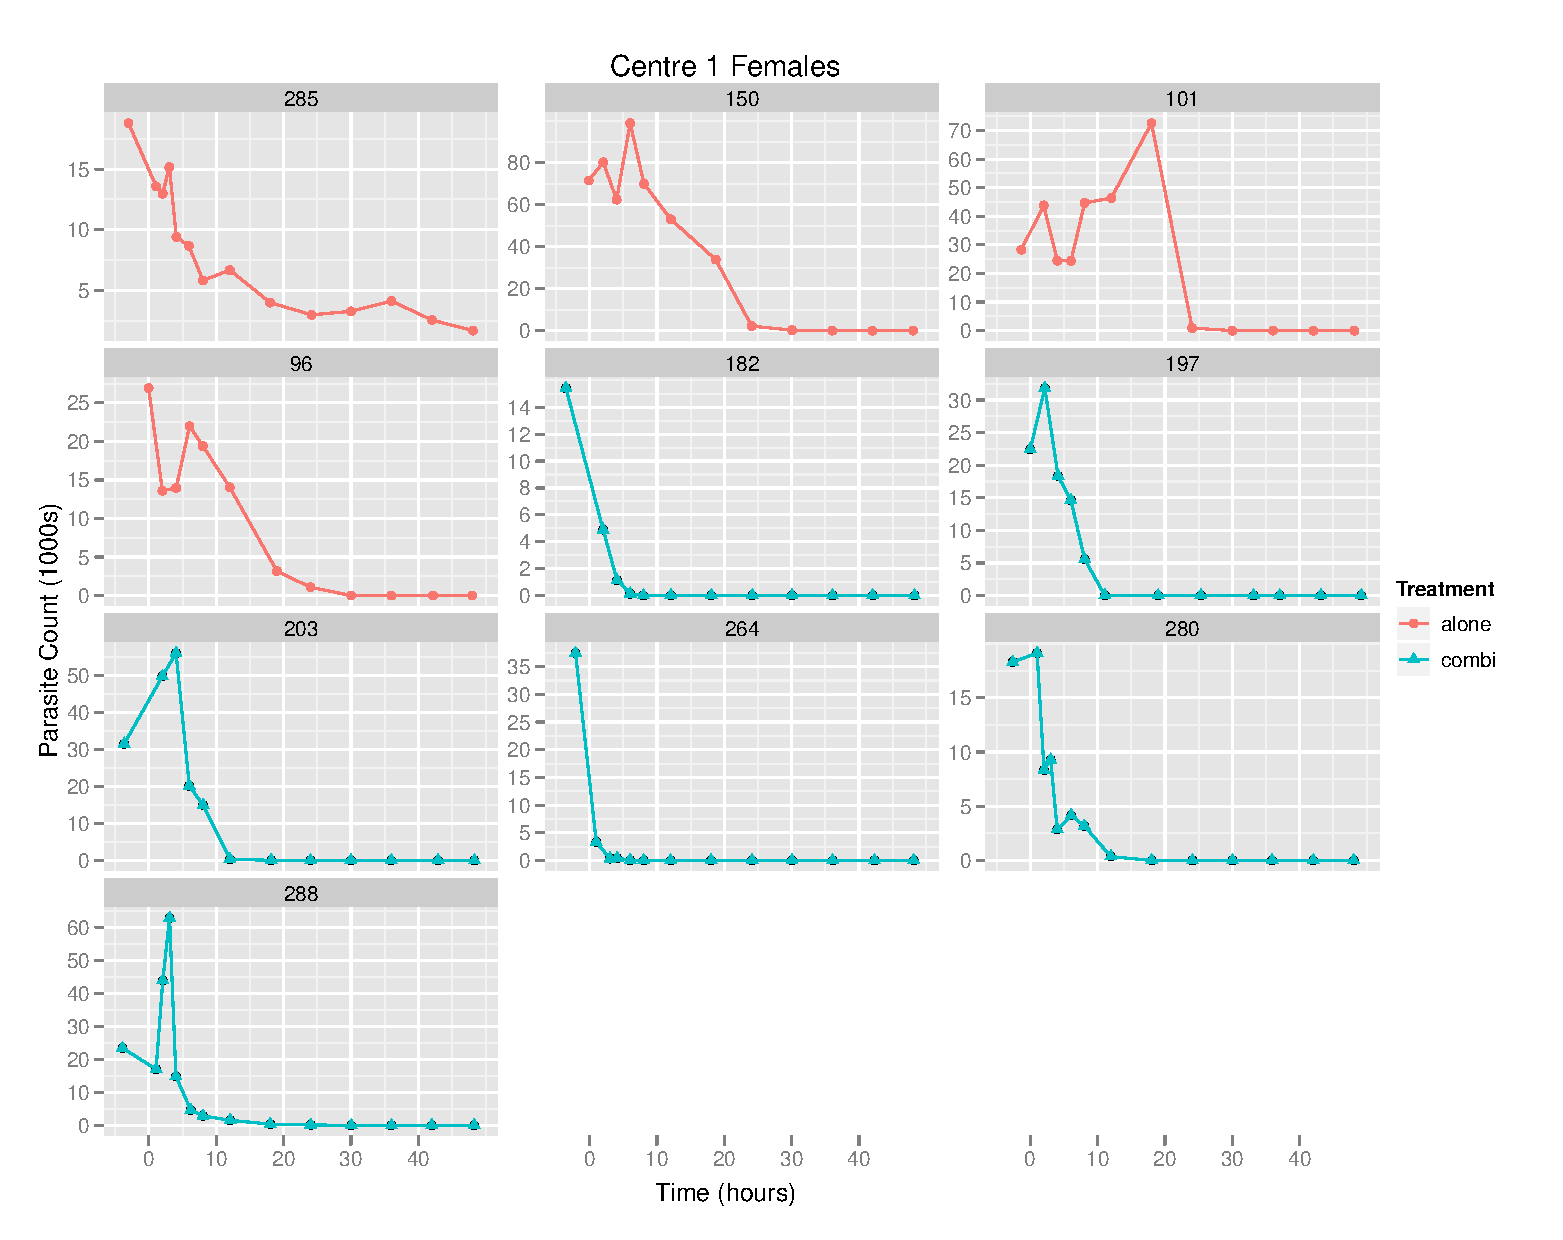
\includegraphics[width=6.1in]{raw1f.eps}
\caption{Parasite count for centre 1 females}\label{raw1F}
\end{figure} 
\begin{figure}[h]
\centering
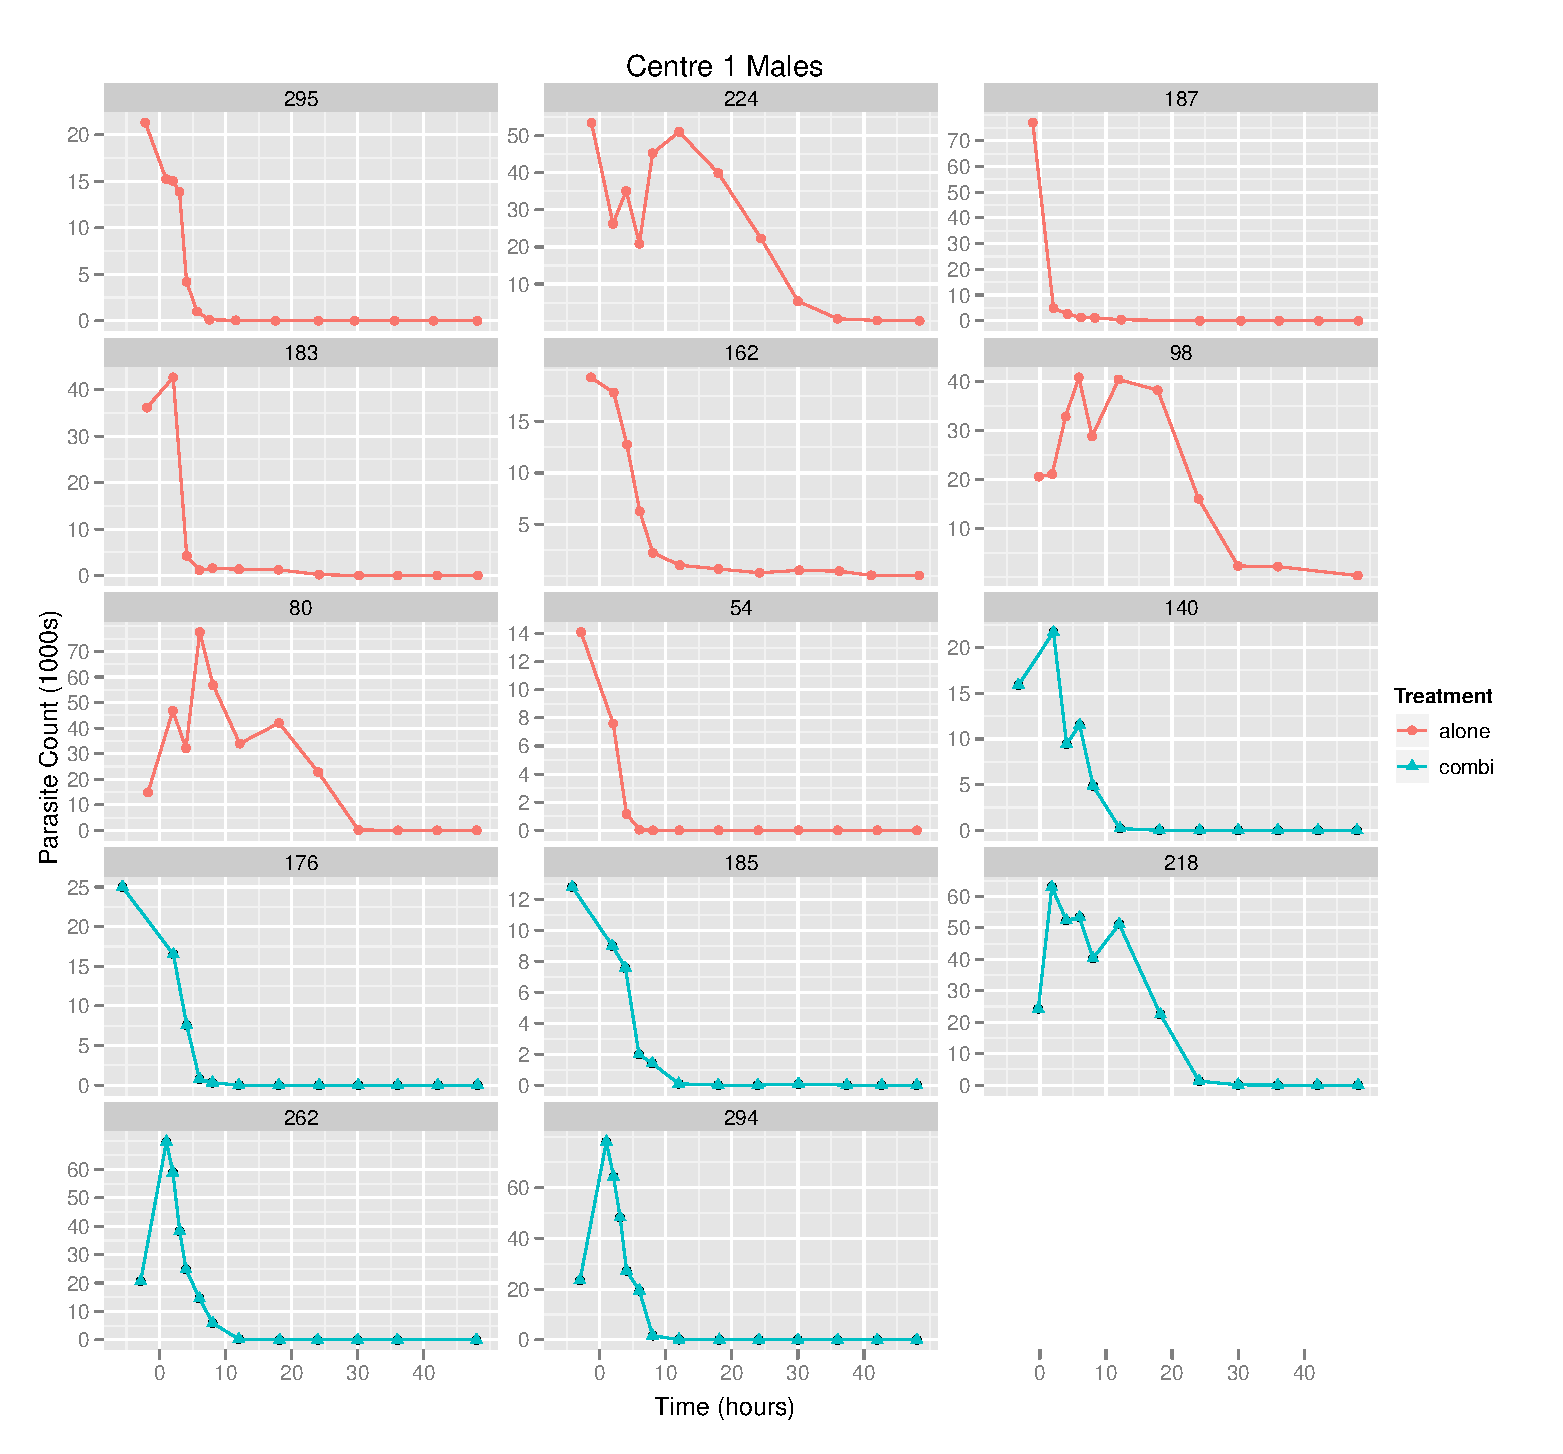
\includegraphics[width=6.1in]{raw1m.eps}
\caption{Parasite count for centre 1 males}\label{raw1M}
\end{figure} 
\begin{figure}[h]
\centering
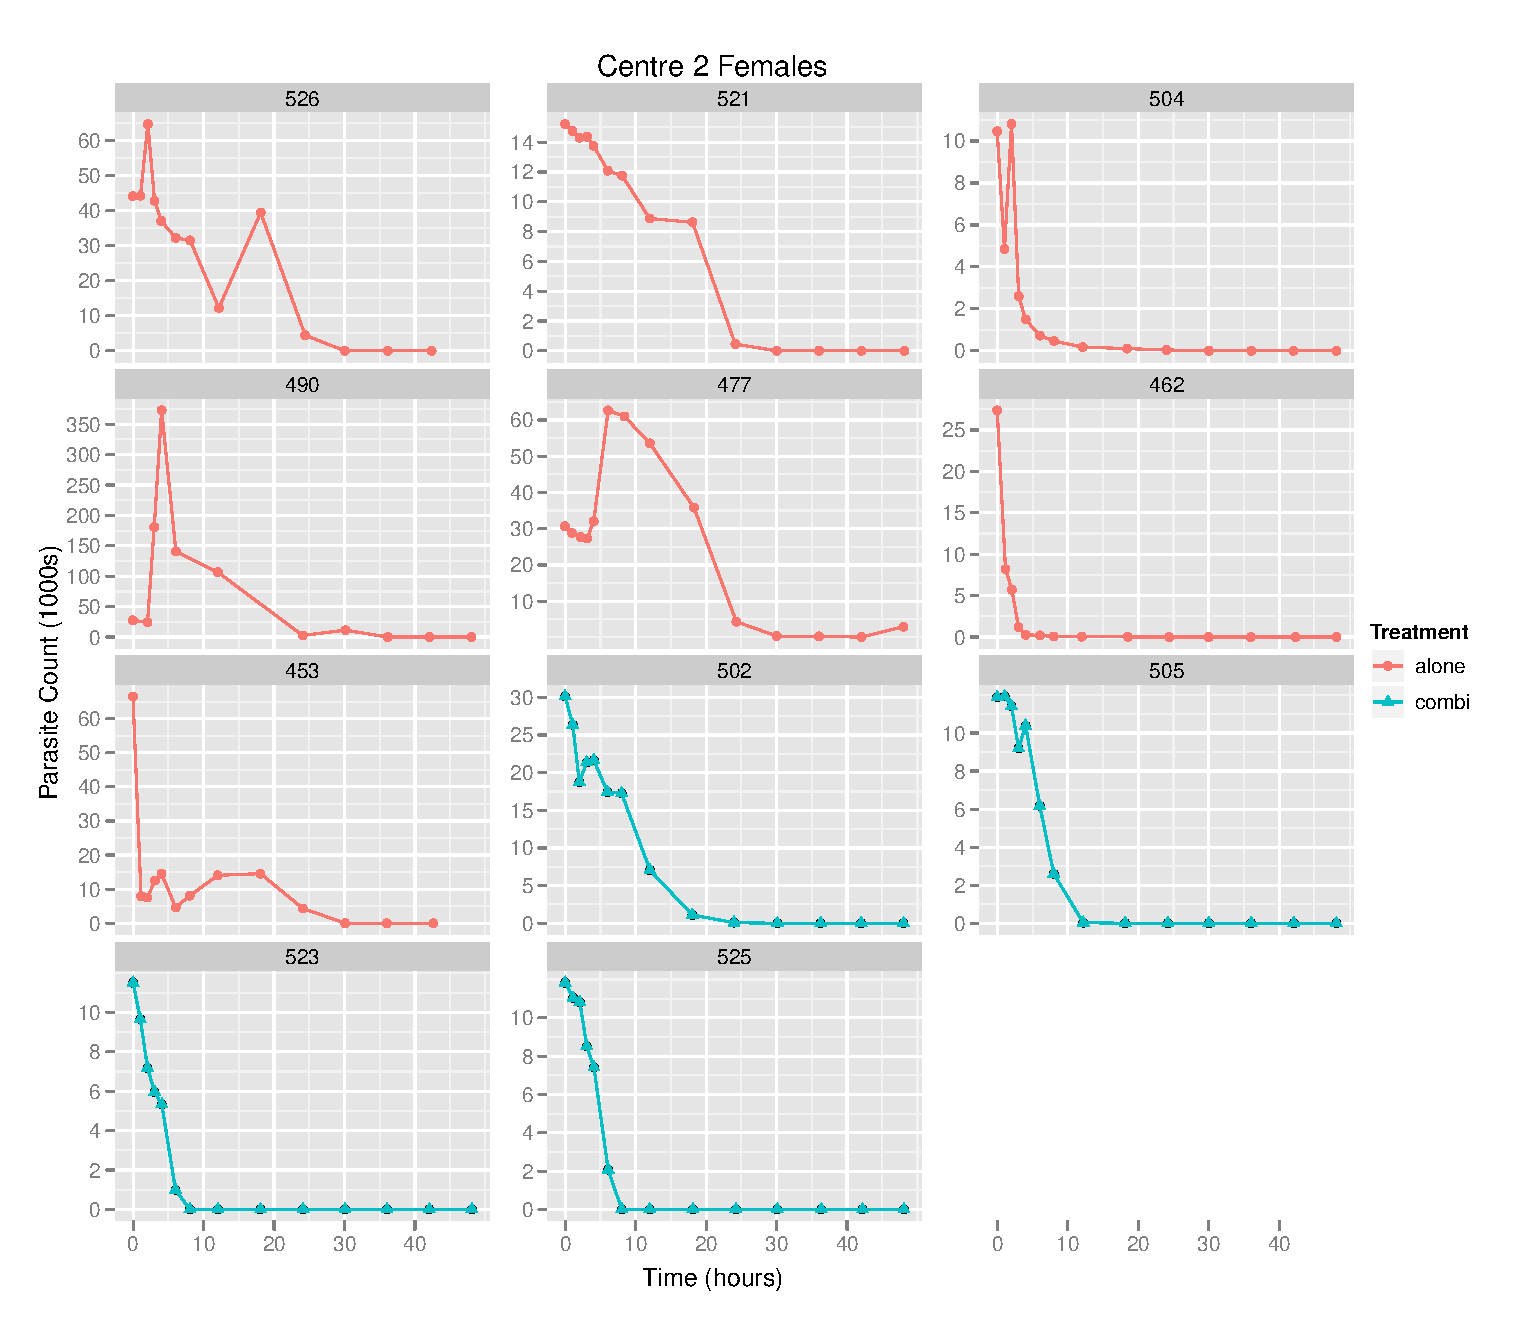
\includegraphics[width=6.1in]{raw2f.eps}
\caption{Parasite count for centre 2 females}\label{raw2F}
\end{figure} 
\begin{figure}[h]
\centering
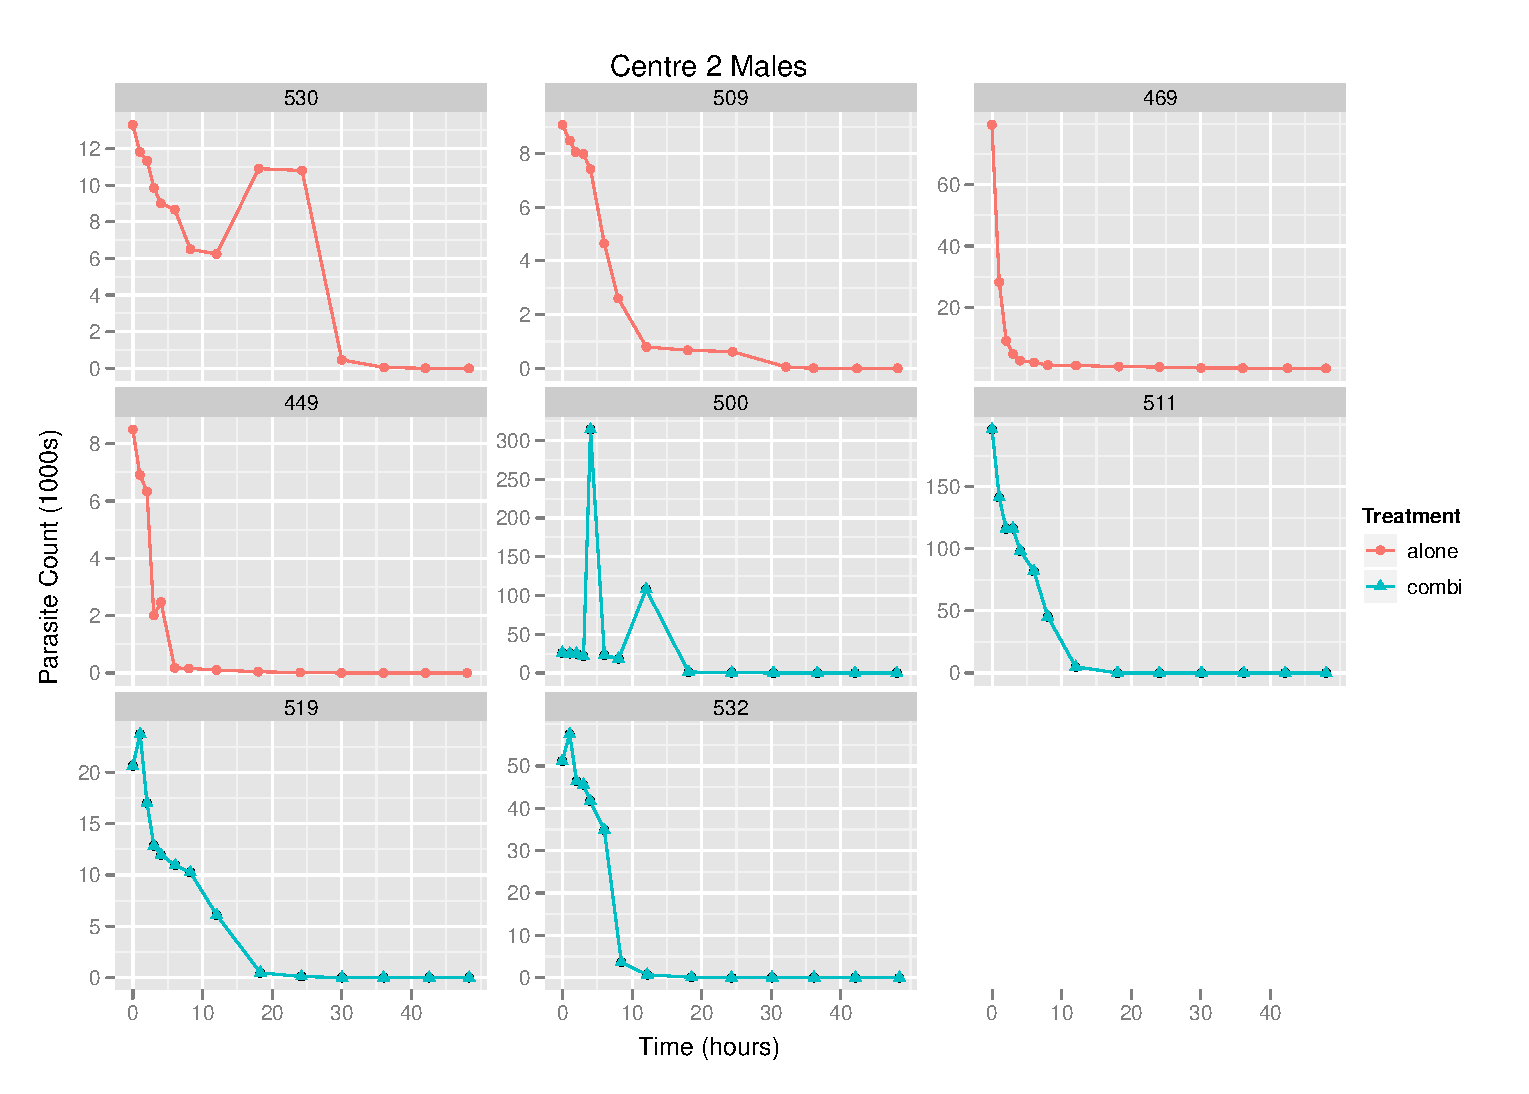
\includegraphics[width=6.1in]{raw2m.eps}
\caption{Parasite count for centre 2 males}\label{raw2M}
\end{figure} 
\subsection{Main features of the data}
Generally, there appears to be a drop in the parasite count from an initial high level to zero or near zero within about 20 to 30 hours from first treatment. In some cases there is a rapid monotonic drop off within 10 hours. In other cases the \textit{recorded} parasite count fluctuates up and down before dropping to zero over a longer period.

\pagebreak
To briefly summarise, the main behaviours observed are:
\begin{itemize}
\item A relatively steep monotonic drop in the count e.g. centre 1 female subjects 182 and 264 (Figure \ref{raw1F}), centre 1 male subjects 187, 162, 54, 176 and 185 (Figure \ref{raw1M}), centre 2 female subjects 462, 523 and 525 (Figure \ref{raw2F}) and centre 2 male subjects 509, 469 and 511 (Figure \ref{raw2M}).

A variation of this type comprises has the parasite count increasing after the first dose before falling e.g. subjects 197 and 203 (Figure \ref{raw1F}) and subjects 262 and 294 (Figure \ref{raw1M}). 
\item A more erratic and slower drop in the parasite count e.g. centre 1 female subjects 285 and 96 (Figure \ref{raw1F}), centre 1 male subjects 295 and 140 (Figure \ref{raw1M}) and centre 2 female subjects 521, 502 and 505 (Figure \ref{raw2F}). 
\item The parasite count seems to fluctuate about a constant level before falling e.g. centre 1 female subjects 150 and 101 (Figure \ref{raw1F}) and centre 1 male subjects 224, 98, 80 and 218 (Figure \ref{raw1M}). 
\end{itemize}
There are some profiles that we might suspect contain anomalous data such as subject 500 in Figure \ref{raw2M} where there are two unusually high values compared to the main trend. We might suspect that some inconsistency in the counting procedure explains these values rather than the patient's parasite count jumping by a large amount on these occasions. Looking at how the parasite count was obtained should give an insight into potential sources of inconsistency.
\section{Derivation of the Parasite Count}
One of the first questions addressed was whether the parasite count is a true count, and thus Poission statistics would be applicable, or whether it is a derived measurement. Our contact informed us that the method used to arrive at the parasite count values given is broadly as follows.
\begin{enumerate}
 \item A microscopist would choose ``suitable area'' of a slide of blood and work from left to right counting parasites ($N_p$) and white blood cells ($N_w$).
\item If by the time they have counted around 200 white blood cells they have seen less than 10 parasites then they continue counting until they have counted around 500 white blood cells.
\item The number of white blood cells in a $\mu L$ of blood ($\rho_w$) is automatically counted by a machine.
\end{enumerate}
Accordingly the number of parasites in a $\mu L$ of blood (\texttt{parct}) is given by:
$$\mathtt{parct}=\frac{N_p}{N_w}\rho_w$$
and thus we cannot treat this derived measurement as a count for modeling purposes.
\subsection{The Pre-dose parasite count}
We were also informed that the white blood cell count is right skewed and so we might expect that the parasite count per $\mu L$ will be also. Table \ref{predose} shows the pre-treatment parasite counts in the subjects from each test centre and of each sex. It can be seen that for 3 cases the mean is larger than the median meaning that the distributions are right skewed. This is to be expected for non-negative data such as this. When model fitting to this data we may have to choose some transformation of the parasite count such as taking logarithms.

If we perform 3-way ANOVA of the parasite count with sex, centre and treatment as factors we find that there is no evidence of a difference due to these factors.
\begin{table}[h]
\centering
\caption{Pre-dose parasite counts}\label{predose}
\begin{tabular}{|cc|cccccc|}
\hline
Centre&Sex&N&Mean&Median&SD&1st Qu.&3rd Qu.\\\hline
\multirow{2}{*}{001}&M&14&27060&20960&17820.9&16750&24830\\
&F&10&29410&25170&16221.2&19700&30700\\\hline
\multirow{3}{*}{002}&M&8&50540&23290&63679.9&12240&58290\\
%&$M^*$&\textit{7}&\textit{29750}&\textit{20610}&\textit{26436.6}&\textit{11180}&\textit{38580}\\
&F&11&26110&27360&17262.4&11860&30400\\\hline
\end{tabular}
\end{table}
